% This is text associated with the open textbook "Open Electromagnetics"
% See immediately below for author, date
% This work is licensed under the Creative Commons Attribution-ShareAlike 4.0 International License. (CC BY-SA 4.0) 
% To view a copy of the license, visit http://creativecommons.org/licenses/by-sa/4.0/

%ORB TITLE TM Reflection in Non-magnetic Media
%ORB AUTHOR 0        # S.W. Ellingson, Virginia Tech (ellingson@vt.edu)
%ORB DATE 20191120   # yyyymmdd
%ORB ABSTRACT 

\label{m0172_TM_Reflection_Nonmagnetic_Media} % <-- Must match name of this file and module directory name.  Don't mess with this!
\index{transverse magnetic|(}

Figure~\ref{m0172_fObliqueTM} shows a TM uniform plane wave incident on the planar boundary between two semi-infinite material regions.
%
\begin{figure}[b!]
\begin{center}
\pdftooltip{{  % note double braces
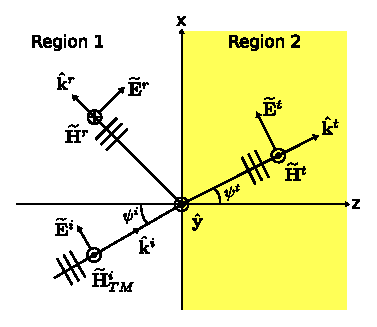
\includegraphics[width=2in]{modules/m0172_fObliqueTM.eps} %,angle=-90,origin=c
% https://commons.wikimedia.org/wiki/File:TM-polarized_upw_incident_on_planar_boundary.svg
}}{For a z-x Cartesian coordinate system, a TE plane wave approaches planar boundary at an oblique angle. The reflected wave in region 1 has magnetic field intensity out of page with electric field i orthogonal to the plane wave and pointing toward the boundary line. The transmitted wave in region 2 has magnetic field intensity out of page with electric field orthogonal to the plane wave and pointing towards the boundary line.}
\end{center}
\centerline{\scriptsize 
\copyright~\hyperref[m0172_fObliqueTM_Credit]{C.\ Wang} 
\href{https://creativecommons.org/licenses/by-sa/4.0/}{CC BY-SA 4.0} 
} 
\caption{
\label{m0172_fObliqueTM}
A transverse magnetic uniform plane wave obliquely incident on the planar boundary between two semi-infinite material regions.
}
\end{figure}
%
In this case, the reflection coefficient is given by:
%
\begin{equation}
\Gamma_{TM} = \frac{-\eta_1\cos\psi^i+\eta_2\cos\psi^t}{+\eta_1\cos\psi^i + \eta_2\cos\psi^t}
\label{m0172_eGTM}
\end{equation}
%
where $\psi^i$ and $\psi^t$ are the angles of incidence and transmission (refraction), respectively; and $\eta_1$ and $\eta_2$ are the wave impedances in Regions~1 and 2, respectively.
Many materials of practical interest are non-magnetic; that is, they have permeability that is not significantly different from the permeability of free space.  In this section, we consider the behavior of the reflection coefficient for this class of materials.

To begin, recall the general form of Snell's law: 
\index{Snell's law}
%
\begin{equation}
\sin{\psi^t} = \frac{\beta_1}{\beta_2}\sin\psi^i
\label{m0172_eSLNM}
\end{equation}
%
In non-magnetic media, the permeabilities $\mu_1$ and $\mu_2$ are assumed equal to $\mu_0$.  Thus:
%
\begin{equation}
\frac{\beta_1}{\beta_2} = \frac{\omega\sqrt{\mu_1\epsilon_1}}{\omega\sqrt{\mu_2\epsilon_2}} = \sqrt{\frac{\epsilon_1}{\epsilon_2}}
\end{equation}
%
Since permittivity $\epsilon$ can be expressed as $\epsilon_0$ times the relative permittivity $\epsilon_r$, we may reduce further to:
%
\begin{equation}
\frac{\beta_1}{\beta_2} = \sqrt{\frac{\epsilon_{r1}}{\epsilon_{r2}}}
\end{equation}
%
Now Equation~\ref{m0172_eSLNM} reduces to:
%
\begin{equation}
\sin{\psi^t} = \sqrt{\frac{\epsilon_{r1}}{\epsilon_{r2}}} \sin\psi^i
\end{equation}
%
Next, note that for any value $\psi$, one may write cosine in terms of sine as follows:
%
\begin{equation}
\cos{\psi} = \sqrt{1-\sin^2{\psi}}
\end{equation}
%
Therefore, 
%
\begin{equation}
\cos{\psi^t} = \sqrt{1-\frac{\epsilon_{r1}}{\epsilon_{r2}} \sin^2\psi^i }
\label{m0172_eCpt}
\end{equation}
%
Also we note that in non-magnetic media
%
\begin{flalign}
\eta_1 &= \sqrt{\frac{\mu_1}{\epsilon_1}} = \sqrt{\frac{\mu_0}{\epsilon_{r1}\epsilon_0}} = \frac{\eta_0}{\sqrt{\epsilon_{r1}}} \\
\eta_2 &= \sqrt{\frac{\mu_2}{\epsilon_2}} = \sqrt{\frac{\mu_0}{\epsilon_{r2}\epsilon_0}} = \frac{\eta_0}{\sqrt{\epsilon_{r2}}} 
\end{flalign}
%
where $\eta_0$ is the wave impedance in free space.
Making substitutions into Equation~\ref{m0172_eGTM}, we obtain:
%
\begin{equation}
\Gamma_{TM} = \frac{-\left(\eta_0/\sqrt{\epsilon_{r1}}\right)\cos\psi^i + \left(\eta_0/\sqrt{\epsilon_{r2}}\right)\cos\psi^t}
                   {+\left(\eta_0/\sqrt{\epsilon_{r1}}\right)\cos\psi^i + \left(\eta_0/\sqrt{\epsilon_{r2}}\right)\cos\psi^t}
\end{equation}
%
Multiplying numerator and denominator by $\sqrt{\epsilon_{r2}}/\eta_0$, we obtain:
%
\begin{equation}
\Gamma_{TM} = \frac{-\sqrt{\epsilon_{r2}/\epsilon_{r1}}\cos\psi^i + \cos\psi^t}
                   {+\sqrt{\epsilon_{r2}/\epsilon_{r1}}\cos\psi^i + \cos\psi^t}
\end{equation}
%
Substituting Equation~\ref{m0172_eCpt}, we obtain:
%
\begin{equation}
\Gamma_{TM} = \frac{-\sqrt{\epsilon_{r2}/\epsilon_{r1}}\cos\psi^i+\sqrt{1-\left(\epsilon_{r1}/\epsilon_{r2}\right)\sin^2\psi^i}}
                   {+\sqrt{\epsilon_{r2}/\epsilon_{r1}}\cos\psi^i+\sqrt{1-\left(\epsilon_{r1}/\epsilon_{r2}\right)\sin^2\psi^i}}
\end{equation}
%
This expression has the advantage that it is now entirely in terms of $\psi^i$, with no need to first calculate $\psi^t$.

Finally, multiplying numerator and denominator by $\sqrt{\epsilon_{r2}/\epsilon_{r1}}$, we obtain:
%
\begin{equation}
\boxed{
\Gamma_{TM} = \frac{-\left(\epsilon_{r2}/\epsilon_{r1}\right)\cos\psi^i+\sqrt{\epsilon_{r2}/\epsilon_{r1}-\sin^2\psi^i}}
                   {+\left(\epsilon_{r2}/\epsilon_{r1}\right)\cos\psi^i+\sqrt{\epsilon_{r2}/\epsilon_{r1}-\sin^2\psi^i}}
}
\label{m0172_eGTMi}
\end{equation}

Using Equation~\ref{m0172_eGTMi}, we can easily see how different combinations of material affect the reflection coefficient.
First, we note that when $\epsilon_{r1}=\epsilon_{r2}$ (i.e., same media on both sides of the boundary), $\Gamma_{TM}=0$ as expected.
When $\epsilon_{r1}>\epsilon_{r2}$ (e.g., wave traveling in glass toward air), we see that it is possible for $\epsilon_{r2}/\epsilon_{r1}-\sin^2\psi^i$ to be negative, which makes $\Gamma_{TM}$ complex-valued.  This results in \emph{total internal reflection}, 
\index{total internal reflection}
and is addressed in another section.
When $\epsilon_{r1}<\epsilon_{r2}$  (e.g., wave traveling in air toward glass), we see that $\epsilon_{r2}/\epsilon_{r1}-\sin^2\psi^i$ is always positive, so $\Gamma_{TM}$ is always real-valued.

Let us continue with the $\epsilon_{r1}<\epsilon_{r2}$ condition.
Figure~\ref{m0172_fTMnmG} shows $\Gamma_{TM}$ plotted for various combinations of media over all possible angles of incidence from 0 (normal incidence) to $\pi/2$ (grazing incidence).
%
\begin{figure} % <--- "[b]" for first figure in section *only*; delete for 2nd and subsequent figures
\begin{center}
\pdftooltip{{  % note double braces
\includegraphics[width=2in,angle=-90,origin=c]{modules/m0172_fTMnmG.eps} 
% https://commons.wikimedia.org/wiki/File:M0003_fBarMagnet.svg
}}{Three concave curves from the highest coefficient to lowest have ratios 2, 10, and 100. The curves approach the zero angle value as the ratio increases.}
\end{center}
%\centerline{\scriptsize 
%\copyright~\hyperref[m0003_fBarMagnet_Credit]{Y.\ Qin} 
%\href{https://creativecommons.org/licenses/by/3.0/}{CC BY 3.0} 
%} % \centerline 
\caption{
\label{m0172_fTMnmG}
The reflection coefficient $\Gamma_{TM}$ as a function of angle of incidence $\psi^i$ for various media combinations, parameterized as $\epsilon_{r2}/\epsilon_{r1}$.
}
\end{figure}
%
We observe:
%
%%%%%%%%%%%%%%%%%%%%%%%%%%%%%%%%%%%%%%%%%%%%%%%
%ORB HIGHLIGHT
\begin{mdframed}[backgroundcolor=yellow!20,nobreak=true] 
In non-magnetic media with $\epsilon_{r1}<\epsilon_{r2}$, 
$\Gamma_{TM}$ is real-valued and increases from a negative value for normal incidence to $+1$ as $\psi^i$ approaches grazing incidence.
\end{mdframed}
%%%%%%%%%%%%%%%%%%%%%%%%%%%%%%%%%%%%%%%%%%%%%%%
%
Note that at any particular angle of incidence, $\Gamma_{TM}$ trends toward $-1$ as $\epsilon_{r2}/\epsilon_{r1}\to\infty$.
In this respect, the behavior of the TM component is similar to that of the TE component. 
In other words: As $\epsilon_{r2}/\epsilon_{r1}\to\infty$, the result for both the TE and TM components are increasingly similar to the result we would obtain for a perfect conductor in Region~2. 

Also note that when $\epsilon_{r1}<\epsilon_{r2}$, $\Gamma_{TM}$ changes sign from negative to positive as angle of incidence increases from 0 to $\pi/2$.
This behavior is quite different from that of the TE component, which is always negative for $\epsilon_{r1}<\epsilon_{r2}$.
The angle of incidence at which $\Gamma_{TM}=0$ is referred to as \emph{Brewster's angle},
\index{Brewster's angle}
which we assign the symbol $\psi^i_B$.
Thus:
%
\begin{equation}
\boxed{
\psi^i_B \triangleq \psi^i ~~\mbox{at which}~~ \Gamma_{TM}=0
}
\end{equation}
%
In the discussion that follows, here is the key point to keep in mind:
%
%%%%%%%%%%%%%%%%%%%%%%%%%%%%%%%%%%%%%%%%%%%%%%%
%ORB HIGHLIGHT
\begin{mdframed}[backgroundcolor=yellow!20,nobreak=true] 
Brewster's angle $\psi^i_B$ is the angle of incidence at which $\Gamma_{TM}=0$.
\end{mdframed}
%%%%%%%%%%%%%%%%%%%%%%%%%%%%%%%%%%%%%%%%%%%%%%%

Brewster's angle is also referred to as the \emph{polarizing angle}.
\index{polarizing angle}
The motivation for the term ``polarizing angle'' is demonstrated in Figure~\ref{m0172_fPolarizingAngle}.
%
\begin{figure} % <--- "[b]" for first figure in section *only*; delete for 2nd and subsequent figures
\begin{center}
\pdftooltip{{  % note double braces
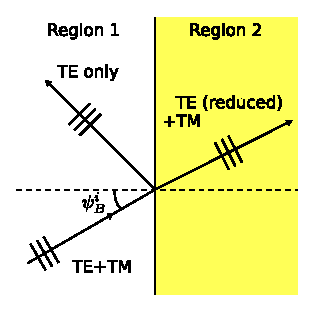
\includegraphics[width=2in]{modules/m0172_fPolarizingAngle.eps} 
% https://commons.wikimedia.org/wiki/File:Reflection_of_plane_wave_incidence_angle_equals_polarizing_angle.svg
}}{A plane wave of TE plus TM approaches the boundary at small psi superscript i subscript capital B. The reflection wave is TE only. The transmitted is TE (reduced) plus TM.}
\end{center}
\centerline{\scriptsize 
\copyright~\hyperref[m0172_fPolarizingAngle_Credit]{C.\ Wang} 
\href{https://creativecommons.org/licenses/by-sa/4.0/}{CC BY-SA 4.0} 
} % \centerline 
\caption{
\label{m0172_fPolarizingAngle}
Reflection of a plane wave with angle of incidence $\psi^i$ equal to the polarizing angle $\psi^i_B$. 
Here the media are non-magnetic with $\epsilon_{r1}<\epsilon_{r2}$.
}
\end{figure}
%
In this figure, a plane wave is incident with $\psi^i=\psi^i_B$.  
The wave may contain TE and TM components in any combination. 
Applying the principle of superposition, we may consider these components separately.
The TE component of the incident wave will scatter as reflected and transmitted waves which are also TE.
However, $\Gamma_{TM}=0$ when $\psi^i=\psi^i_B$, so the TM component of the transmitted wave will be TM, but the TM component of the reflected wave will be zero.
Thus, the total (TE$+$TM) reflected wave will be purely TE, regardless of the TM component of the incident wave.
This principle can be exploited to suppress the TM component of a wave having both TE and TM components.
This method can be used to isolate the TE and TM components of a wave.

{\bf Derivation of a formula for Brewster's angle.}
Brewster's angle for any particular combination of non-magnetic media may be determined as follows.
$\Gamma_{TM}=0$ when the numerator of Equation~\ref{m0172_eGTMi} equals zero, so:
%
\begin{equation}
-R\cos\psi^i_B+\sqrt{R-\sin^2\psi^i_B} = 0
\end{equation}
%
where we have made the substitution $R\triangleq\epsilon_{r2}/\epsilon_{r1}$ to improve clarity.
Moving the second term to the right side of the equation and squaring both sides, we obtain:
%
\begin{equation}
R^2\cos^2\psi^i_B = R-\sin^2\psi^i_B
\end{equation}
%
Now employing a trigonometric identity on the left side of the equation, we obtain:
%
\begin{flalign}
R^2\left(1-\sin^2\psi^i_B\right) &= R-\sin^2\psi^i_B \\
         R^2 -R^2 \sin^2\psi^i_B &= R-\sin^2\psi^i_B  \\
\left(1-R^2\right)\sin^2\psi^i_B &= R - R^2 
\end{flalign}
%
and finally
%
\begin{equation}
\sin\psi^i_B = \sqrt{ \frac{ R - R^2 }{ 1-R^2 } }
\label{m0172_eBA1}
\end{equation}
%
Although this equation gets the job done, it is possible to simplify further.
Note that Equation~\ref{m0172_eBA1} can be interpreted as a description of the right triangle shown in Figure~\ref{m0172_fBAtriangle}. 
%
\begin{figure} % <--- "[b]" for first figure in section *only*; delete for 2nd and subsequent figures
\begin{center}
\pdftooltip{{  % note double braces
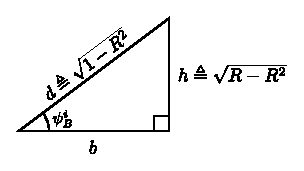
\includegraphics[width=2in]{modules/m0172_fBAtriangle.eps} 
% https://commons.wikimedia.org/wiki/File:Brewster%E2%80%99s_angle_for_non-magnetic_media.svg
}}{A right triangle with hypotenuse labeled small d to be equal to the square root of the quantity one minus capital r squared. The height is small h to be equal to the square root of the quantity capital r minus capital r squared. The base is small b. The angle between the hypotenuse and base is small psi superscript small i and subscript capital b.}
\end{center}
\centerline{\scriptsize 
\copyright~\hyperref[m0172_fBAtriangle_Credit]{C.\ Wang} 
\href{https://creativecommons.org/licenses/by-sa/4.0/}{CC BY-SA 4.0} 
} % \centerline 
\caption{
\label{m0172_fBAtriangle}
Derivation of a simple formula for Brewster's angle for non-magnetic media. 
}
\end{figure}
%
In the figure, we have identified the length $h$ of the vertical side and the length $d$ of the hypotenuse as:
%
\begin{flalign}
h &\triangleq \sqrt{R-R^2} \\
d &\triangleq \sqrt{1-R^2}
\end{flalign}
%
The length $b$ of the horizontal side is therefore
%
\begin{equation}
b = \sqrt{d^2-h^2} = \sqrt{1-R}
\end{equation} 
%
Subsequently, we observe
%
\begin{equation}
\tan\psi^i_B = \frac{h}{b} = \frac{\sqrt{R-R^2}}{\sqrt{1-R}} = \sqrt{R}
\end{equation}
%
Thus, we have found
%
\begin{equation}
\boxed{
\tan\psi^i_B = \sqrt{\frac{\epsilon_{r2}}{\epsilon_{r1}}}
}
\label{m0172_eBA}
\end{equation}

%%%%%%%%%%%%%%%%%%%%%%%%%%%%%%%%%%%%%%%%%%%%%%%
%ORB EXAMPLE
~\\ \begin{example} 
\begin{mdframed}[backgroundcolor=brown!20,linecolor=brown!20]\raggedright
Polarizing angle for an air-to-glass interface.
\\~\\
A plane wave is incident from air onto the planar boundary with a glass region.
The glass exhibits relative permittivity of 2.1. 
The incident wave contains both TE and TM components. 
At what angle of incidence $\psi^i$ will the reflected wave be purely TE?\\
~\\

\noindent
{\bf Solution.}
Using Equation~\ref{m0172_eBA}:
%
\begin{equation}
\tan\psi^i_B = \sqrt{\frac{\epsilon_{r2}}{\epsilon_{r1}}} = \sqrt{\frac{2.1}{1}} \cong 1.449
\end{equation}
%
Therefore, Brewster's angle is $\psi^i_B\cong$ \underline{$55.4^{\circ}$}.
This is the angle $\psi^i$ at which $\Gamma_{TM}=0$.
Therefore, when $\psi^i=\psi^i_B$, the reflected wave contains no TM component and therefore must be purely TE.
\end{mdframed}
%
\end{example}
%%%%%%%%%%%%%%%%%%%%%%%%%%%%%%%%%%%%%%%%%%%%%%%

%%%%%%%%%%%%%%%%%%%%%

{\bf Additional Reading:}
\begin{itemize}
\item ``\href{https://en.wikipedia.org/wiki/Brewster's_angle}{Brewster's angle}'' on Wikipedia.
\end{itemize}

\index{transverse magnetic|)}
